\subsection{Our Techniques}

\paragraph{Endemic Security.} When defining malicious security of an OT, one defines an ideal functionality $\OOT$. An OT is called secure, if for any adversary against the OT scheme, there exists an adversary interacting with \OOT producing the same output. Classically, $\OOT$ either receives the OT strings $s_0$, $s_1$ as input from the sender or samples them uniformly at random and outputs them to the sender. But there are also OTs where the receiver can determine the OT strings or even both parties could influence how the OT strings are generated. We distinguish four main security notions.
\begin{description}
\item[Uniform Message Security:] The ideal functionality $\OOT^{\U}$ samples the OT strings uniformly and outputs them to sender and one to the receiver.
\item[Sender Chosen Message Security:] The ideal functionality $\OOT^{\send}$ receives the OT strings from the sender and outputs one of the strings to the receiver.
\item[Receiver Chosen Message Security:] The ideal functionality $\OOT^{\rec}$ receives one of the OT strings from the receiver, samples the other one uniformly at random and outputs the strings to the sender.
\item[Endemic Security] If the sender is malicious, it chooses both strings. If the receiver is malicious, it chooses one of the strings. All strings that are not choosen yet, are sampled uniformly by the functionality $\OOT^{\E}$. The sender obtains both strings and the receiver obtains one. 
\end{description}

Notice that endemic security gives the weakest security guarantees, no matter whether the receiver or the sender is malicious, the malicious party can always determine the output distribution. Uniform message security gives very strong security guarantees since a malicious party can never influence the distribution.
     
%imps: {lemma:is_a}

\paragraph{Relations Between Security Notions.} We show on one hand that an OT with uniform message security is also secure with respect to all other security notions. On the other hand, uniform, sender and receiver chosen message security imply endemic security. Still, there are very simple transformations from an endemically secure OT to an OT that achieves any of the other security notions. Though we remark that uniform message security implies and therefore requires a secure coin tossing protocol. In \figureref{fig:OTrelations}
\begin{figure}
\centering
\begin{tikzpicture}
\node (U) at (4,4) {Uniform Message Security};
\node (SC) at (0,2) {$\OOT^\send$-Security};
\node (RC) at (8,2) {$\OOT^\rec$-Security};
\node (E) at (4,0) {Endemic Security};
\node (TC) at (3,2) {Coin Tossing};
\node (M) at (5,2) {};
\pgfextractangle{\angle}{SC}{RC}
\draw [-implies,double equal sign distance] (U) --node [midway,above,rotate=0]{$\scalebox{0.8}{\lref{lemma:is_a}}\quad\quad$} (SC);
\pgfextractangle{\angle}{U}{RC}
\draw [-implies,double equal sign distance] (U) --node [midway,above,rotate=0]{$\quad\quad\scalebox{0.8}{\lref{lemma:is_a}}$} (RC);
\pgfextractangle{\angle}{SC}{E}
\draw [-implies,double equal sign distance] (SC) --node [midway,above,rotate=0]{$\quad\quad\scalebox{0.8}{\lref{lemma:is_a}}$} (E);
\pgfextractangle{\angle}{E}{RC}
\draw [-implies,double equal sign distance] (RC) --node [midway,above,rotate=0]{$\scalebox{0.8}{\lref{lemma:is_a}}\quad\quad$} (E);
\pgfextractangle{\angle}{TC}{U}
\draw [->, thick] (U) to [out=240,in=90] node [midway,left,rotate=0]{$\scalebox{0.8}{\lref{lem:OTtoC}}$}(TC);
\draw [-, thick] (E) to [out=60,in=270] (5,2);
\pgfextractangle{\angle}{U}{M}
\draw [->, thick] (5,2) to [out=90,in=300] node [pos=-0.05,left,rotate=0]{$\quad\scalebox{0.8}{\lref{lem:EtoU}}$} (U);
\draw [-, thick] (TC) to [out=0,in=300] (4.655,3);
\pgfextractangle{\angle}{SC}{E}
\draw [->, thick] (E) to [out=180,in=270] node [midway,below,rotate=0]{$\scalebox{0.8}{\lref{lem:EtoS}}\quad\enspace$} (SC);
\pgfextractangle{\angle}{E}{RC}
\draw [->, thick] (E) to [out=0,in=270] node [midway,below,rotate=0]{$\enspace\quad\scalebox{0.8}{\lref{lem:EtoR}}$} (RC);
\end{tikzpicture}
\label{fig:OTrelations}
\caption{
The figure depicts the different security notions of OT and their relations. $A\Rightarrow B$ denotes that security $A$ implies security $B$. $A\rightarrow B$ denotes that any OT realizing security $A$ can be efficiently transformed into an OT realizing security $B$.
}
\end{figure}
we give an overview over these implications and transformations. 

We also show that endemic OT is weaker than the other notions but at the same time this allows a minimal round complexity of a single round. More precisely, we show that there is no one round OT that achieves sender or receiver chosen message security.

\paragraph{From Key Agreement to OT.} A common strategy to construct OT from PKE is to use a PKE where the public keys form a group \cite{C:PeiVaiWat08}, which we will denote with $(\G,\oplus)$. By giving a challenge $c$ and forcing the receiver to generate two public keys $\pk_0$ and $\pk_1$ s.t. $c=\pk_0\oplus \pk_1$, he can intuitively only decrypt ciphertexts with respect to one of them. But this does actually not follow from the standard notion of PKE since an adversary could generate $\pk_0$ and $\pk_1$ jointly given $c$. It requires a dual-mode cryptosystem \cite{C:PeiVaiWat08} that is tailored towards this property. Dual-mode cryptosystems are known from DDH, QR and LWE \cite{C:PeiVaiWat08} but is not clear how to extend these results to other assumptions.\footnote{Barreto et al. \cite{EPRINT:BDDMN17b} claim to construct a dual-mode cryptosystem with search hardness from coding based assumptions, but their security analysis has significant gaps, namely it lacks a security reduction.}

Another approach \cite{C:OstRicSca15,cryptoeprint:2018:473} uses specific commitment protocols which forces the receiver to commit to a public key before $c$ is known. The drawback of this approach is that it requires four rounds and the known constructions of such a commitment protocol are not efficient \cite{STOC:Kilian92,C:OstRicSca15}. 

We propose a different solution that uses a novel and simple technique to leverage the power of a random oracle. Rather than choosing two public keys, we ask the receiver to generate two strings $r_0$, $r_1$ in \G. From these strings a sender can generate the public keys $\pk_0=r_0\oplus\H(r_1)$, $\pk_1=r_1\oplus\H(r_0)$ under which he can encrypt the two OT messages $s_0$, $s_1$.
In the actual protocol, the receiver can program $r_b\in \{r_0,r_1\}$ to a public key 
for his choice of $b\in\bits$. He samples $r_{1-b}$ and sets $r_b=\pk\ominus\H(r_{1-b})$.

This technique also allows to extract $s_0$, $s_1$ from a malicious sender by programming the random oracle such that secret keys for both, $\pk_0$ and $\pk_1$ are known. Further, one can extract $b$ from a malicious receiver by programming the random oracle as well. Intuitively, a malicious receiver needs to query either $r_0$ or $r_1$ first. His choice will determine $r_{1-b}$, since all following random oracle queries $q$ can be programmed such that $\H(q)=\pk'-r_{1-b}$ for a public key $\pk'$. If a malicious adversary can learn $s_{1-b}$, he will decrypt a ciphertext for $\pk_{1-b}=r_{1-b}\oplus\H(q)=\pk'$ and be able to break the PKE scheme.

We optimize the protocol further by using a key agreement instead of a PKE scheme. In many settings, the OT messages don't need to be chosen, it is sufficient if they are pseudorandom. Hence, no ciphertext needs to be generated, only the exchanged keys need to be computed. This save in some settings a communication round, e.g. in case of the Diffie-Hellman key exchange \cite{DifHel76}.

\paragraph{Secure OT Extension.} 
In \sectionref{sec:otext} we explore the rich implications endemic security has on efficient 1-out-of-$N$ OT extension along with presenting three new attacks and fixes of existing OT extension protocols\cite{C:KelOrsSch15,RSA:OrrOrsSch17} with Uniform Message security\footnote{\cite{C:KelOrsSch15,RSA:OrrOrsSch17} refer to uniform OT as random OT $\mathcal{F}^{m,\kappa}_{\textsf{ROT}}$}. 
\iffullversion
These protocols are derived from the seminal black-box protocol of Ishia, Kilian, Nissim and Petrank\cite{C:IKNP03}. We note that in all cases the Sender Chosen Message variant of these protocols\cite{C:IKNP03,C:KelOrsSch15,RSA:OrrOrsSch17} are secure. 
\fi
The functionality of 1-out-of-$N$ OT extension allows $\nc\approx\kappa$ instances of 1-out-of-2 OTs to be transformed into $m=\textsf{poly}(\kappa)$ instances of 1-out-of-$N$ OTs. There are several advantages of this transformation 1) $m$ can be polynomial times larger than $\nc$. 2) Only symmetric key cryptography is required which provides a larger performance improvement. 3) In some cases $N$ can be exponential in the security parameter $\kappa$ which we indicate with the use of capital $N$. 

The 1-out-of-2 OTs that are being transformed are referred to as \emph{base OTs}. Existing protocols \cite{C:IKNP03,EC:ALSZ15,C:KelOrsSch15,RSA:OrrOrsSch17} have called for the use of base OTs with the sender chosen message security notion, e.g. $\OOT^\send$. However, we show that this requirement can be relaxed to allow the base OTs to only achieve endemic security. In both cases ($\OOT^\send$ or $\OOT^\E$ base OTs) the OT extension protocol outputs messages that satisfy the Endemic security notion.  Tradition OT extension protocols, e.g. \cite{C:IKNP03,EC:ALSZ15,C:KelOrsSch15}, then apply the $\Pi^{\send}_{1,N}$ transform from \figureref{fig:protoSendOT} to realize the Sender Chosen Message functionality $\OOT^\send$.
\iffullversion
 This observation suggests that more efficient OT extension can be realized by replacing Sender Chosen Message base OTs with Endemic OTs, e.g. our protocol.
\fi
The authors of \cite{C:KelOrsSch15,RSA:OrrOrsSch17} suggest that the $\Pi^{\send}_{1,N}$ transform  can be removed and resulting protocol would satisfy the Uniform Message security notion, but in  \ref{sec:extAttack} we show this to not be the case. 
\iffullversion
In particular, \ref{sec:extAttack} detail three attacks where the first  allows a malicious party to bias the OT messages that they output while the second and third attacks succeed even when base OTs with uniform message security are used. In all cases, the ability to bias the messages violates the ideal functionality which samples them uniformly at random. Therefore, we show that the protocol only achieves Endemic security.

We note that many protocols that utilize Uniform Message security can likely tolerate the weaker notion of Endemic security, e.g. \cite{EC:RinRos17,CCS:RinRos17}.  However, other protocols such as the set inclusion protocol of \cite[Figure 5]{RSA:OrrOrsSch17} are insecure\footnote{The sender set all the OT messages to be the same value and force the receiver to conclude their item is in the sender's set.} when Uniform Message security is not satisfied. 
\fi

\begin{figure}
	\centering
	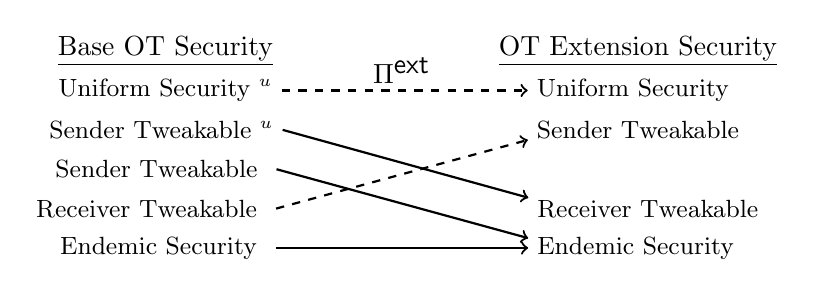
\begin{tikzpicture}[scale=0.5]\small
	\node (pi) at (6,4.5) {\normalsize $\Pi^\textsf{ext}$};
	\node (Base) at (0,5) {\underline{\normalsize Base OT Security}};
	\node (U) at (0,4) {Uniform Security $\OOT^{\U u}$};
	\node (SCu) at (-0.1,3) {Sender Tweakable $\OOT^{\send u}$};
	\node (SC) at (-0.1,2) {Sender Tweakable $\OOT^{\send}$};
	\node (RC) at (-0.35,1) {Receiver Tweakable  $\OOT^{\rec}$};
	\node (E) at (-0.05,0) {Endemic Security  $\OOT^{\E}$};
	
	
	\node (Ext) at (12,5) {\underline{\normalsize OT Extension Security}};
	\node (EU) at (12,4) {Uniform Security $\OOT^{\U}$};
	\node (ESC) at (12.13,3) {Sender Tweakable $\OOT^{\send}$};
	\node (ERC) at (12.38,1) {Receiver Tweakable  $\OOT^{\rec}$};
	\node (EE) at (12.07,0) {Endemic Security  $\OOT^{\E}$};
%	\draw [-implies,double equal sign distance] (U) -- (SC);
%	\draw [-implies,double equal sign distance] (U) -- (RC);
%	\draw [-implies,double equal sign distance] (SC) -- (E);
%	\draw [-implies,double equal sign distance] (RC) -- (E);
	\draw [->, thick, dashed] (U) -- (EU);
	\draw [->, thick] (E) -- (EE);
	\draw [->, thick] (SCu.east) -- (ERC.175);
	\draw [->, thick, dashed] (RC.east) -- (ESC.185);
	\draw [->, thick] (SC.east) -- (EE.175);
	
%	\draw [-, thick] (5,2.5)-- (TC);
%	\draw [->, thick] (E) .. controls (1,0.75) .. (SC);
%	\draw [->, thick] (E) .. controls (7,0.75) .. (RC);
	\end{tikzpicture}
	\label{fig:OTExtrelations}
	\caption{
		The figure depicts the implication different Base OT security notions (\definitionref{def:otSec}) have on the result OT extension protocol.  $A\rightarrow B$ denotes that any OT realizing security $A$ can be efficiently transformed by $\Pi^\textsf{ext}$ into an OT extension realizing security $B$, where $\Pi^\textsf{ext}$ is the protocol of \figureref{fig:otExt} such that $\OOT$ is the left hand side oracle. The dashed arrows are the same expect $\Pi^{\textsf{ext}}$ must be slightly modified. 
	}
\end{figure}

From endemic OT extension uniform message security can be achieved in several ways. One solution is the black-box transformation $\Pi^\U_{1,N}$ of \figureref{fig:uniformOT} which lifts an OT protocol with Endemic security to satisfy Uniform Message security. However, this would require additional rounds and significant communication. We demonstrate an alternative solution which replaces the base OTs with a protocol that satisfies Uniform Message, Uniform Selection security $\OOT^{\U u}$ and prove that this yields an OT extension protocol with Uniform Message security without the need to modify the extension protocol. More generally, \figureref{fig:OTExtrelations} shows the relation between different base OT security notions and the resulting OT extension message security. 
\iffullversion
For example, the protocols of \cite{C:IKNP03,EC:ALSZ15,C:KelOrsSch15} perform
$$
\OOT^\send \xrightarrow{\Pi^{\textsf{ext}}} \OOT^\E \xrightarrow{\Pi^{\send}_{1,2}} \OOT^\send
$$
where $\Pi^\textsf{ext}$ is their respective extension protocol up to hashing.
\fi

In addition, \sectionref{sec:extIdealCipher} details new OT extension protocols that can efficiently be realized in the ideal cipher model. These protocol are inspired by existing implementation \cite{libOTe,KOS,EMP} but are provably secure. Unfortunately, these existing implementation improperly apply the ideal cipher model which could be leverage by a malicious receiver to fully break \emph{all} OT messages. In addition to providing provable security, the protocols that we introduce and formalize are roughly 10 times more efficient than their counter parts in the random oracle model.
%\textcolor{red}{mention ideal cipher optimization}


\paragraph{Implementation.} We instantiate our OT protocol with the Diffie-Hellman key exchange. We show how the security loss can be reduced using the random self-reducibility of the DDH assumption. 
We also instantiate it based on the Kyber key exchange \cite{EPRINT:BDKLLS17,NISTPQC-R1:CRYSTALS-KYBER17}. This is a proof of concept instantiation that shows that our framework is very agile in terms of assumptions and allows to obtain post-quantum security efficiently. 

We give implementations and benchmarks for two OT protocols based on DDH and one based on LWE as well as five implementations of OT extension protocols. We compare our results with the OTs of Chou \& Claudio \cite{LC:ChoOrl15} and Naor \& Pinkas \cite{SODA:NaoPin01} and the OT extensions of Keller, Orsini \& Scholl \cite{C:KelOrsSch15}. 